In order to corroborate \sysname{}, we aim to study two questions:
% \begin{itemize}[leftmargin=*]
% \begin{itemize}
%     \item \textbf{Q1}: Can \sysname{} be successfully applied to problems where task distribution in the training domain is partially shifted from the task distribution in the testing domain?
%     \item \textbf{Q2}: Instead of learning task weights, can \sysname{} deal with problems where data instances with noisy labels are used during the meta-training stage by learning weights in an instance-level scheme?
% \end{itemize}
\textbf{Q1}: Can \sysname{} be successfully applied to problems where task distribution in the training domain is partially shifted from the task distribution in the testing domain?
\textbf{Q2}: Instead of learning task weights, can \sysname{} deal with problems where data instances with noisy labels are used during the meta-training stage by learning weights in an instance-level scheme?


To answer these questions, we conduct the following experiments: (1) Mix OOD tasks with the meta-training tasks to evaluate the task-level weighting scheme of \sysname{} and (2) corrupt the labels of some training samples to evaluate the instance-level weighting scheme of \sysname{}. We follow the classification experiments in \cite{finn2017model} to do few-shot learning to evaluate both the task-level and the instance-level weighting schemes. In addition, a synthetic regression experiment is conducted for the task-level weighting scheme as well. Due to the space limitation, we list synthetic regression experiments and detailed experimental settings in Appendix \ref{app:addExp}. We performed all the experiments using PyTorch, and the code is available at \url{https://bit.ly/3s3gARc}. 

% To study robustness of our model regarding the OOD scenario in the task weighting scheme, we separately design supervised learning experiments with regression and classification settings. Noisy labels experiments are designed to validate the proposed \sysname{} in the instance weight scheme.

\textbf{Datasets.} We use \textbf{\textit{mini}-ImageNet}~\citep{ravi2016optimization}, \textbf{SVHN}~\citep{netzer2011reading}, \textbf{FashionMNIST}~\citep{xiao2017fashion} datasets in our experiments. For the task-level weighting scheme, \textbf{\textit{mini}-ImageNet} is considered as the ID tasks source ($\mathcal{D}_{in}$). Both the \textbf{SVHN} and the \textbf{FashionMNIST} datasets are used as OOD tasks source ($\mathcal{D}_{out}$) for \textbf{\textit{mini}-ImageNet}. For instance-level weighting, \textbf{\textit{mini}-ImageNet} is considered with corrupted labels. Additional details about datasets are given in Appendix \ref{app:exp_details}.
% We consider \textbf{mini-ImageNet}~\citep{ravi2016optimization} as in-distribution data ($\mathcal{D}_{in}$), \textbf{SVHN}~\citep{netzer2011reading} and \textbf{FashionMNIST}~\citep{xiao2017fashion} as out-of-distribution outliers ($\mathcal{D}_{out}$) for \textit{mini}-ImageNet.

\subsection{Task-level Weighting for OOD Tasks}
\label{sec:exp_task-level}
\vspace{-1mm}
% \subsection{Few-shot Classification with Outliers}
\textbf{Settings.} We implement image classification experiments in 5-way, 3-shot (5-shot) settings. And we use a model with similar backbone architecture given in ~\citep{vinyals2016matching,finn2017model} for all baselines. We consider  a total of 20,000 training tasks containing both ID and OOD tasks where the split of ID and OOD tasks is determined by OOD ratio(0.3, 0.6, and 0.9 in this setting). At each iteration, ID tasks and OOD tasks will be sampled according to the OOD ratio. We sample the ID tasks (meta-training, meta-validation, and meta-test) from the \textbf{\textit{mini}-ImageNet} dataset and sample OOD tasks from the \textbf{SVHN} or the \textbf{FashionMNIST} dataset.  We process all images to be of size 84$\times$84$\times$3. As mentioned before, in the task-level weighting, all the data instances in a task share the same weight, reducing the weight hyper-parameters count. To further reduce them, we use the K-means clustering method to cluster the tasks and assign a single weight value to all the same cluster tasks. 
% Hyper-parameters are shown in Appendix~\ref{app:addExp}.

% \textbf{Experiment setting:} We implement image classification experiments for 5-way 3-shot and 5-way 5-shot settings. In this experimental setting, we sample all ID tasks from a single dataset \textbf{mini-ImageNet}~\citep{ravi2016optimization} that is considered as in-distribution data ($\mathcal{D}_{in}$). We test for OOD settings using the datasets \textbf{SVHN}~\citep{netzer2011reading} and \textbf{FashionMNIST}~\citep{xiao2017fashion} as OOD tasks sources ($\mathcal{D}_{out}$) for mini-ImageNet. We use 20000 training tasks, and the number of OOD tasks in training tasks is determined based on the OOD ratio. We test the effectiveness of our \sysname{} algorithm for different OOD ratios of 0.3, 0.6, and 0.9. We use a Task Weighting Scheme where all the data instances in a task share the same weight. To further reduce the number of weight hyperparameters that need to be estimated, we use the Kmeans clustering method to cluster the tasks such that all tasks in a cluster share a single weight value. 
% In addition to MAML~\citep{finn2017model}, we compare the proposed \sysname{} with several competing methods in the problem that when OOD tasks are mixed in the meta-training stage. Intuitively,

\textbf{Baselines.} In addition to \textbf{MAML}, we have \textbf{MAML-OOD-RM} which basically removes the OOD tasks during meta-training and hence is a skyline to our model. \textbf{MMAML}~\citep{vuorio2019multimodal} leverages the strengths of meta-learners by identifying the mode of the task distribution and modulating the meta-learned prior in the parameter space. \textbf{B-TAML}~\citep{lee2020l2b} uses relocated initial parameters for new arriving tasks to handle OOD tasks. We adapted \textbf{L2R}~\citep{ren2018learning} to assign weights for different tasks and optimize these weights through stochastic gradient descent. We consider \textbf{Transductive Fine-tuning}~\citep{dhillon2019baseline} as a baseline where we finetune the parameters of the model that is obtained by adding a new classifier on top of a pre-trained deep network, which is pre-trained on support and query sets of the meta-training set, using the meta-test set's support and unlabeled query set.
% Comparison results are shown in the Table~\ref{tab:ood-classification}. 

\begin{table*}[t!]
% \footnotesize
% \vspace{-3mm}
    \small
    
    % \vspace{-3mm}
    \centering
    \begin{center}
    \vspace{-3mm}
    \begin{tabular}{l c c c | ccc}
        \toprule
         & \multicolumn{3}{c}{\textbf{5-way 3-shot}} & \multicolumn{3}{|c}{\textbf{5-way 5-shot}}\\
        
        % \Xhline{2\arrayrulewidth}
        % &\multicolumn{3}{c}{\textbf{5-way 3-shot}} \\
        Noise Ratio & 20\% & 30\% & 50\% & 20\% & 30\% & 50\%  \\
        \midrule
        MAML-Noise-RM & $60.2\scriptstyle{\pm 0.02}$ & $59.35\scriptstyle{\pm 0.01}$ & $58.21\scriptstyle{\pm 0.71}$ & $61.2\scriptstyle{\pm 0.21}$ & $60.3\scriptstyle{\pm 0.32}$ & $59.1\scriptstyle{\pm 0.68}$ \\
        \hline
        MAML    & $54.8\scriptstyle{\pm 0.64}$ & $53.9\scriptstyle{\pm 1.10}$ & $51.8\scriptstyle{\pm 0.12}$ & $59.2\scriptstyle{\pm 0.28}$ & $57.6\scriptstyle{\pm 0.36}$ & $53.5\scriptstyle{\pm 0.48}$   \\
        \sysname{} (ours) & $\textbf{55.24}\scriptstyle{\pm 0.72}$ & $\textbf{54.7}\scriptstyle{\pm 1.20}$ & $\textbf{53.68}\scriptstyle{\pm 0.21}$ & $\textbf{59.6}\scriptstyle{\pm 0.54}$ & $\textbf{58.16}\scriptstyle{\pm 0.87}$ & $\textbf{55.61}\scriptstyle{\pm 1.32}$ \\
        \bottomrule 
        % \Xhline{2\arrayrulewidth}
    \end{tabular}
\vspace{-3mm}
\end{center}
\vspace{-1mm}
\caption{Test accuracies on \textbf{\textit{mini}-Imagenet} with 20\%, 30\%, and 50\% flipped noisy labels during the meta-training phase.}
\label{tab:noise}
\end{table*}

\begin{figure}[!t]
\vspace{-3mm}
%\captionsetup[subfigure]{aboveskip=-1pt,belowskip=-2pt}
    \centering
    \begin{subfigure}[b]{0.23\textwidth}
        \centering
        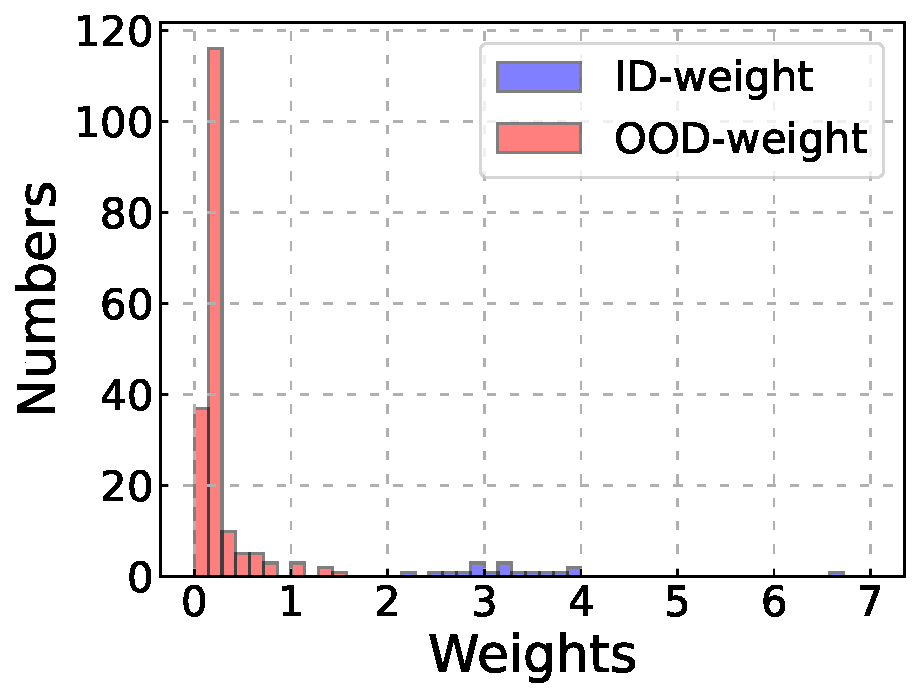
\includegraphics[width=\linewidth, height=2.8cm]{figs/5-Way-3-Shot-ood90.pdf}
        \caption{5-way 3-shot}
    \end{subfigure}
    \begin{subfigure}[b]{0.23\textwidth}
        \centering
        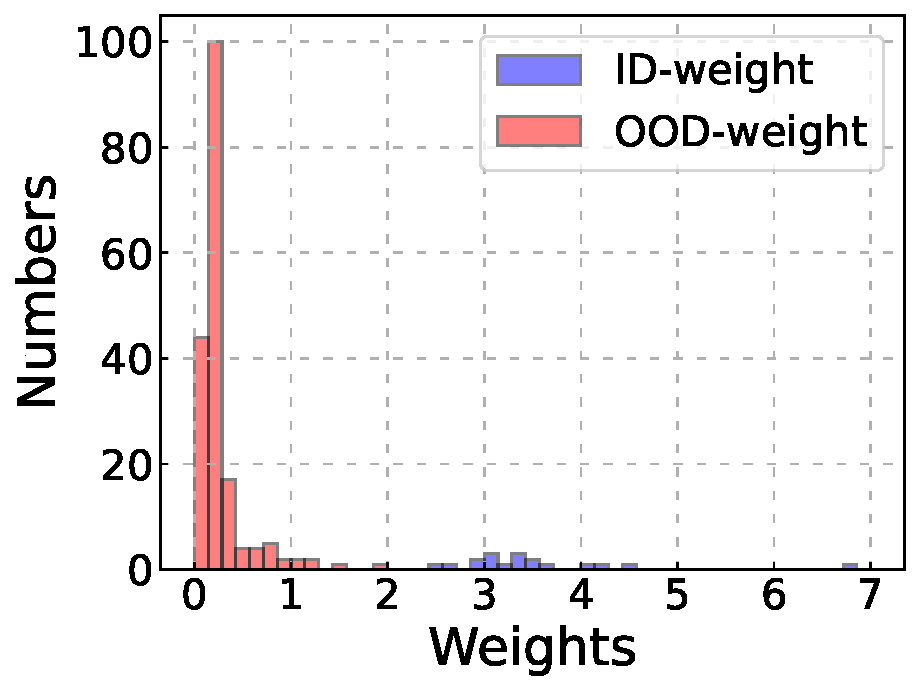
\includegraphics[width=\linewidth, height=2.8cm]{figs/5-Way-5-Shot-ood90.pdf}
        \caption{5-way 5-shot}
    \end{subfigure}
    \vspace{-2mm}
    \caption{Task weight distribution under 90\% ratio (SVHN).}
    \label{fig:weights histogram}
% \vspace{-3mm}
\end{figure}

\textbf{Results.} Results in Table~\ref{tab:ood-classification} show that \sysname{} significantly outperforms all baseline techniques and achieves performance competitive to the skyline method (MAML-OOD-RM) in the experiment of SVHN as OOD. For FashionMNIST OOD, \sysname{} still outperforms all baseline techniques for 60\% and 90\% ratio. For 30\% ratio, the first-order approximation, \sysname{}-FO, has the best accuracy, and \sysname{}'s accuracy is also comparable. Besides, the variance of \sysname{} is smaller than \sysname{}-FO, which means \sysname{} is more stable than \sysname{}-FO and \sysname{} still has the best performance overall. From the perspective of training time, we observed that \sysname{} takes $\mathbf{1.7 \times}$ and \sysname{}-FO takes $\mathbf{1.4 \times}$ the time taken by MAML for training. Figure~\ref{fig:weights histogram} shows weight distribution for OOD and ID tasks under 90\% ratio when SVHN is viewed as the OOD dataset for 5-way 3-shot (5-shot) settings after the meta-training phase. Both settings show that OOD tasks have much smaller weights than ID tasks: the weights belonging to OOD tasks approximately range from 0 to 1; however, the assigned weights for ID tasks are from 2 to 5, sometimes going up to 7. 
% (There are 200 weights because 200 clusters are used.) 

To showcase the weights adaptation process during the training phase, we plot the weights trend as the iterations progress under the 30\% OOD ratio (SVHN) in Figure~\ref{fig:svhn_wt_itera}. 
% Figure~\ref{fig:svhn_wt_itera} (a) and (b) represent 5-way, 3-shot, and 5-way, 5-shot, respectively. 
The Blue (Red) curve denotes the mean weights for ID (OOD) tasks. The shade reflects the variance of weights. Results show that the mean weight assigned to ID tasks would increase as the iterations progress, whereas the weights assigned to OOD tasks remain close to zero, which validates the effectiveness of the \sysname{}.

\begin{figure}[!t]
\vspace{-5mm}
%\captionsetup[subfigure]{aboveskip=-1pt,belowskip=-2pt}
    \centering
    \begin{subfigure}[b]{0.23\textwidth}
        \centering
        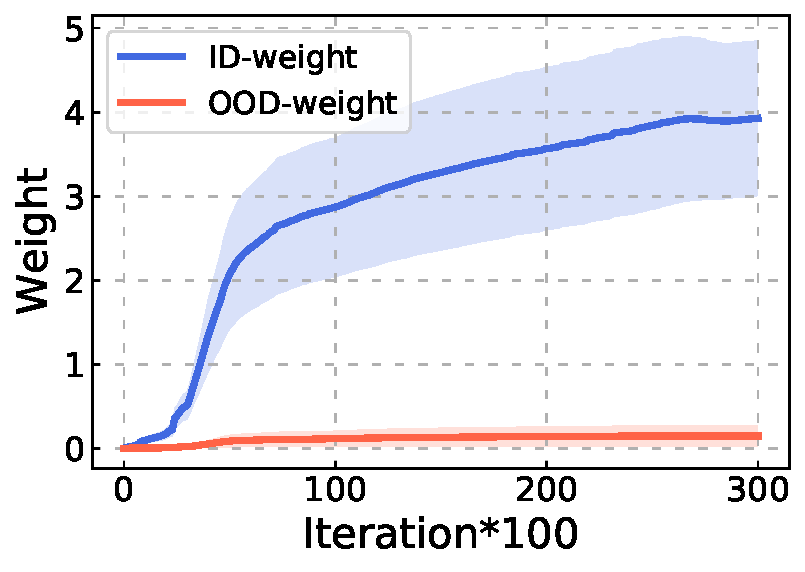
\includegraphics[width=\textwidth]{figs/svhn_5w3s_03.pdf}
        \caption{5-way 3-shot}
    \end{subfigure}
    \begin{subfigure}[b]{0.23\textwidth}
        \centering
        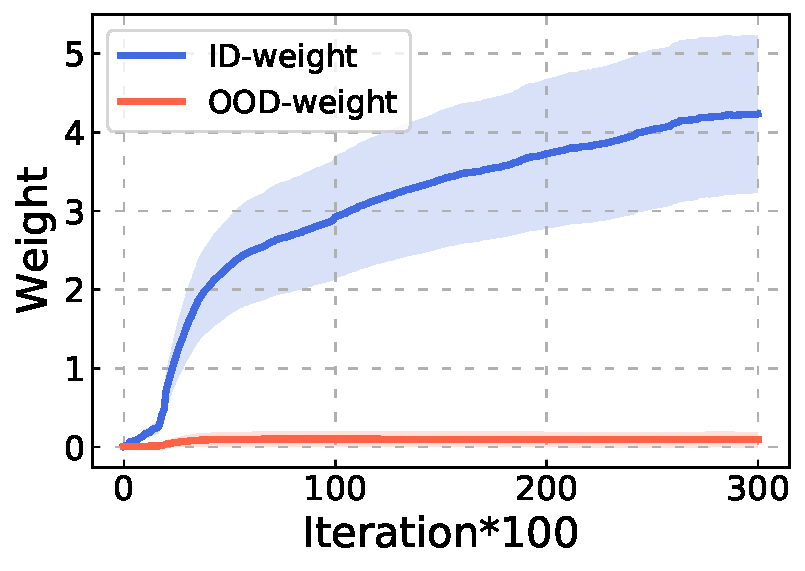
\includegraphics[width=\linewidth]{figs/svhn_5w5s_03.pdf}
        \caption{5-way 5-shot}
    \end{subfigure}
    \vspace{-3mm}
    \caption{Weights trend as the iterations progress for 30\% SVHN OOD experiment}
    \label{fig:svhn_wt_itera}
%\vspace{-8mm}
\end{figure}
\vspace{-1.5ex}

\subsection{Instance-level Weighting For Noisy Labels}
\label{sec:exp_instance-level}
\vspace{-1mm}
Similar to OOD experiments, we implement 5-way 3-shot (5-shot) experiments to evaluate the instance-level weighting scheme. We conduct experiments on noisy labels generated by randomly corrupting the original labels in \textbf{\textit{mini}-ImageNet}. Specifically, different percentages (20\%,30\%, 50\%) of training samples are selected randomly to flip their labels to simulate the noisy corrupted samples.  Intuitively, a deep model robust to noise tries to ignore the data with noisy labels. Note that data containing noisy labels only exist in the meta-training stage. Hyper-parameters are shown in Appendix~\ref{app:addExp}. 

\textbf{Baselines.} We compare our \sysname{} with the following baselines: (1) \textbf{MAML-Noise-RM} serves as a skyline. It is simply modified from MAML, and we manually fix zero weights to instances with noisy labels. (2) \textbf{MAML}.

\textbf{Results.} From the results shown in Table~\ref{tab:noise}, we can conclude that \sysname{} performs better than MAML with high accuracies. 
Furthermore, to circumvent overfitting and reduce computational complexity due to the weight matrix's high dimension, we group instance weights with 200 clusters by K-means, where instances in each cluster share the same weight initialized at 0.005. 

% (2) \textbf{Co-teaching+MAML} \cite{han2018co} is a learning paradigm for combating with noisy labels, in which two deep neural networks are trained simultaneously and let them teach each other given every mini-batch. (3) \textbf{INCV+MAML} \cite{chen2019understanding} adopts the Co-teaching strategy which takes full advantage of the identified samples which is randomly split using cross-validation to train DNNs robustly against noisy labels. (4) \textcolor{red}{\textbf{B-TAML}.???}

\begin{figure}[!t]
\vspace{-3mm}
%\captionsetup[subfigure]{aboveskip=-2pt,belowskip=-2pt}
    \centering
    \begin{subfigure}[b]{0.23\textwidth}
        \centering
         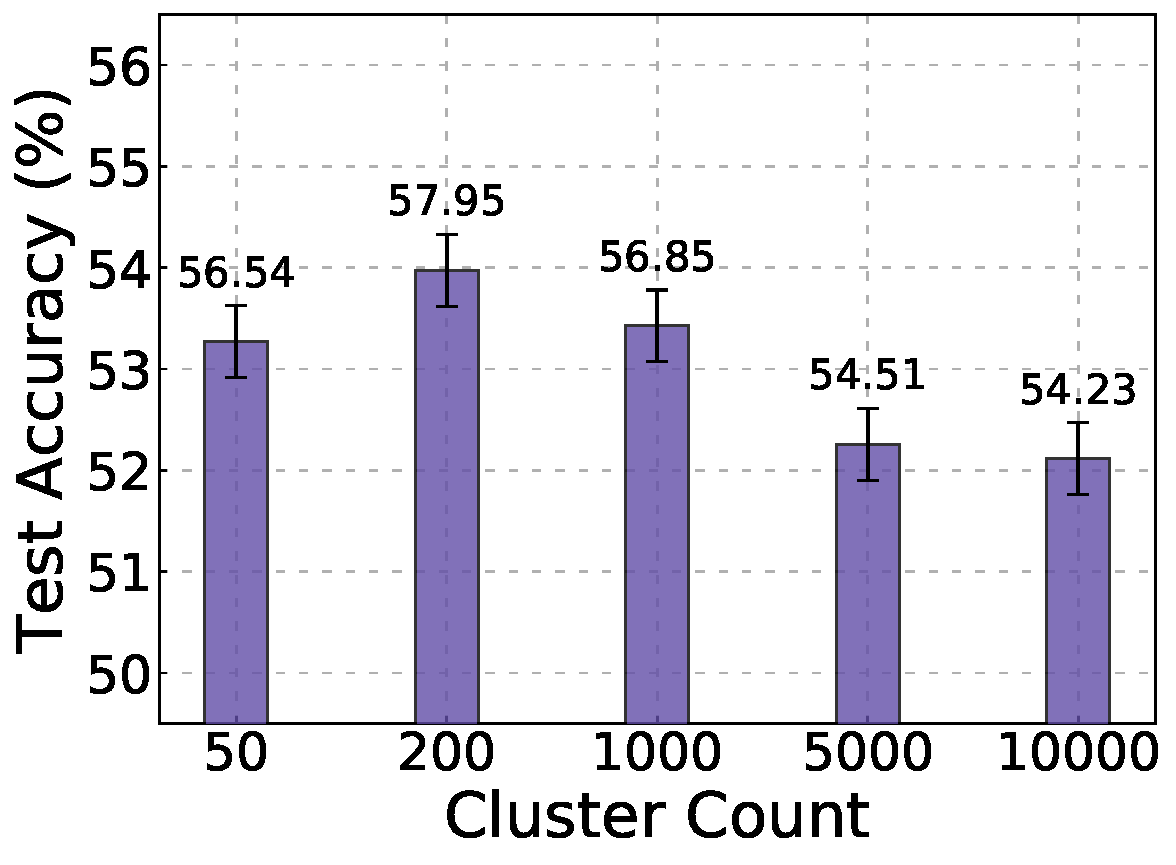
\includegraphics[height=2.9cm]{figs/bar_plot_with_error_bars.pdf}
         \caption{FashionMNIST (90\%)}
         \label{fig:cluster_ablation}
    \end{subfigure}
    \begin{subfigure}[b]{0.23\textwidth}
        \centering
         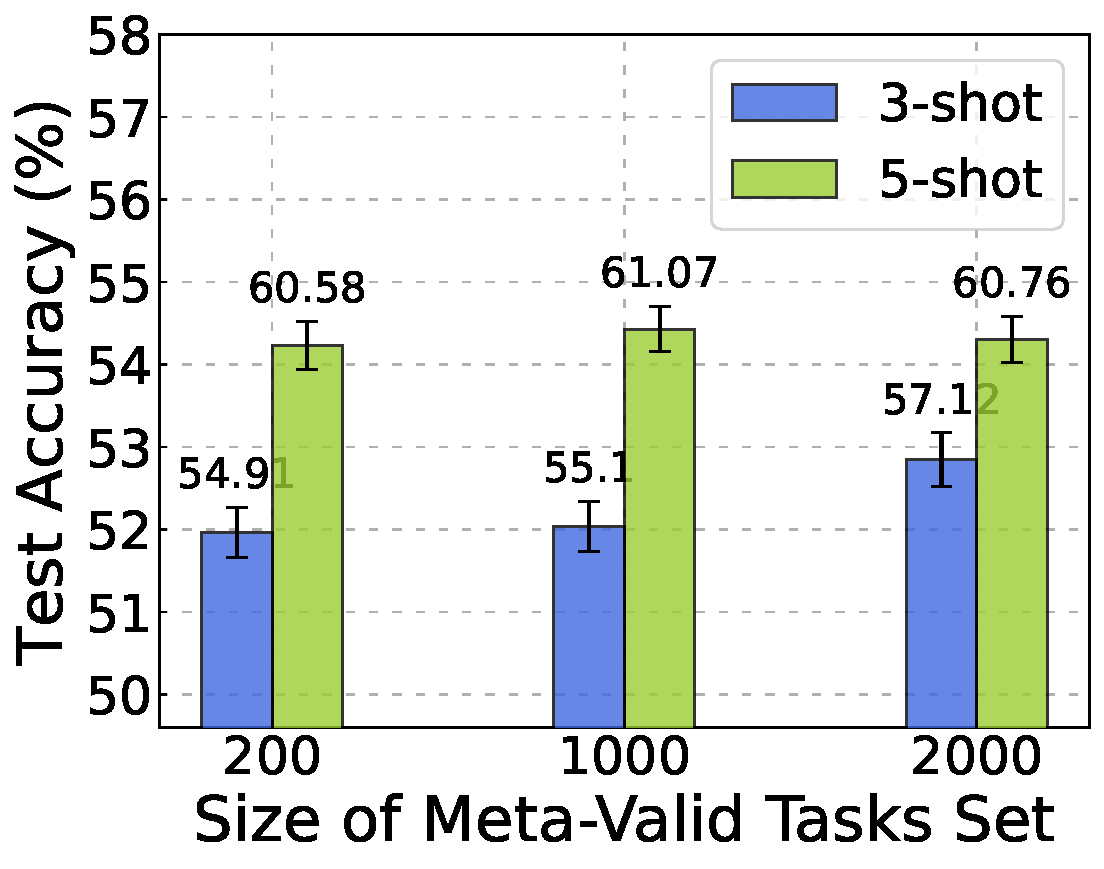
\includegraphics[height=3cm]{figs/bar_plot_valid_tasks_size.pdf}    
         \caption{SVHN (30\%)}
         \label{fig:validation_set}
    \end{subfigure}
    \vspace{-3mm}
    \caption{(a) shows accuracies under 90\% FashionMNIST OOD level with different cluster values, (b) shows accuracies under 30\% SVHN OOD level with different sizes of meta-validation tasks set.}
% \vspace{-3mm}
\end{figure}

\subsection{Sensitivity Analysis}
We perform an ablation study to determine how the number of hyper-parameters and meta-validation sets' size can affect the \sysname{} algorithm's performance. To that extent, we evaluate the \sysname{} algorithm's performance using a different number of clusters in a 5-way 5-shot 90\% FashionMNIST OOD setting. Figure~\ref{fig:cluster_ablation} shows test accuracies versus different numbers of clusters. We observed the best performance when the cluster count is 200. From Figure~(\ref{fig:cluster_ablation}), it is evident that the test accuracy decreases with an increase in the number of clusters that need to be determined. Contrarily, using a tiny number of clusters will also decrease the performance due to decreased clustering efficiency. We used 200 clusters for all our experiments. We also evaluate \sysname{} algorithm's performance using different sizes of the meta-validation set in 5-way 3-shot (5-shot) 30\% SVHN OOD setting. Figure~(\ref{fig:validation_set}) shows that \sysname{} algorithm performs well even when the meta-validation set size is tiny(i.e., 1\% of meta-training set).